\chapter{基于问题分解的多跳长文本阅读理解}
% 摘要:SeqDecomposer, StepDecomposer
% 什么是多跳阅读理解
多跳机器阅读理解是指利用多个相关文档段落进行多次推理,以实现对复杂问题的理解和回答。
相对于常规的单跳机器阅读理解,多跳机器阅读理解需要综合运用文本中的信息,以及常识和推理能力。
% 多跳阅读理解一般用到什么技术
一般来说,多跳阅读理解通常使用基于图神经网络的方法,以及基于检索的方法。
其中,图卷积网络、图注意力网络和图循环网络通过邻接矩阵建立文档间多个句子或实体之间的联系。
基于检索的方法类似于第三章提到的方法,利用文本匹配模型得到与问题相关的文档,然后进行阅读理解。
% 这些技术的缺点
然而,这些模型不擅长寻找支持证据,因为它们缺乏进行真正的多跳推理的能力。
目前的多跳阅读理解模型往往是利用了快捷方式进行求解,这意味着模型无需实际执行必要的推理步骤即可回答问题。
% 本文提出了什么方法,及其大致步骤
因此,本文基于问题分解的思想,提出了两种相关方法SeqDecomposer和StepDecomposer,用来将复杂的多跳问题分解为多个简单的单跳问题。
然后利用这些单跳问题,依次检索出相关文档作为支持证据,并对这些文档进行阅读理解,以获取每个子问题以及最终的答案。
% 实验结果
本章在多跳阅读理解数据集MuSiQue上进行了实验。
实验结果表明,SeqDecomposer和StepDecomposer与现有的检索式基线模型相比,在证据F1的性能上取得了不错的提升。

\section{引言}
% 介绍多跳阅读理解
多跳阅读理解\cite{Yang2018HotpotQAAD}(Multi-hop Reading Comprehension,MH-RC)是指需要在多个相关文档段落中进行多次推理,以实现对复杂问题的理解和回答。
相较于单跳阅读理解,多跳阅读理解更接近于人类的语言推理能力,具有广泛的应用前景,但也具有极大的挑战性。
如图~\ref{tab:5-1}~所示,给出了一个多跳阅读理解数据集MuSiQue的一个例子。
例如,对于一个多跳问题“Who is the president of ... ?”,需要采取方法将其分解为四个子问题,每个子问题都不存在多跳的复杂关系。
对于每个单跳问题,需要在给定的文档集合中找到对应的文档,并从文档中抽取答案。
在该示例中,每个子问题的答案又会重新作用于下一个问题。

\begin{table}[htbp]
    \centering
    \begin{tabular}{p{420pt}}
    \hline
    {\bfseries 相关文档:} \\
    文档13: BULLET::::- On 4 March 2006, Lion Air Flight 8987, a McDonnell Douglas MD-82, crashed after landing at Juanda International Airport. Reverse thrust was used during landing, although the left thrust reverser was stated to be out of service. This caused the aircraft to veer to the right and skid off the runway, coming to rest about from the approach end of the runway. There were no fatalities, but the aircraft was badly damaged and later written off. \\
    <译文:Aga Kagans会奴役Boyars> \\
    文档3: Cathay Pacific Flight 780 was a flight from Surabaya Juanda International Airport in Indonesia to Hong Kong International Airport on 13 April 2010. There were 309 pass       engers and a crew of 13 on board. As Flight 780 neared Hong Kong the crew were unable to change the thrust output of the engines. The aircraft, an Airbus A330-342, landed at almost twice the speed of a        normal landing, suffering minor damage. The 57 passengers who sustained injuries were hurt in the ensuing slide evacuation; one of them received serious injuries. \\
    <译文:Boyars和Aga Kagans会引发战争 > \\
    文档14: The Indonesia\u2013Timor Leste Commission on Truth and Friendship was a truth commission established jointly by the governments of Indonesia and East Timor in August 2       005. The commission was officially created to investigate acts of violence that occurred around the independence referendum held in East Timor in 1999 and sought to find the \"conclusive truth\" behind        the events. After holding private hearings and document reviews, the commission handed in the final report on July 15, 2008 to the presidents of both nations, and was fully endorsed by Indonesian Presid       ent Susilo Bambang Yudhoyono, providing the first acknowledgement by the government of Indonesia of the human rights violations committed by state institutions in Timor. The commission is notable for be       ing the first modern truth commission to be bilateral. \\
    <译文:Aga Kagans会离开Flamme,找到更好的星球> \\
    文档11: Democratic Republic of Timor - Leste Rep\u00fablika Demokr\u00e1tika Tim\u00f3r Lorosa'e (Tetum) Rep\u00fablica Democr\u00e1tica de Timor - Leste (Portuguese) Flag Coa       t of arms Motto: Unidade, Ac\u00e7\u00e3o, Progresso (Portuguese) Unidade, Asaun, Progresu (Tetum) (English: ``Unity, Action, Progress '') Anthem: P\u00e1tria (Portuguese) (English:`` Fatherland'') Capi       tal and largest city Dili 8 \u00b0 20 \u2032 S 125 \u00b0 20 \u2032 E \ufeff / \ufeff 8.34 \u00b0 S 125.34 \u00b0 E \ufeff / - 8.34; 125.34 Coordinates: 8 \u00b0 20 \u2032 S 125 \u00b0 20 \u2032 E \ufef       f / \ufeff 8.34 \u00b0 S 125.34 \u00b0 E \ufeff / - 8.34; 125.34 Official languages Tetum Portuguese National languages 15 languages (show) Atauru Baikeno Bekais Bunak Fataluku Galoli Habun Idalaka Kawa       imina Kemak Makalero Makasae Makuva Mambai Tokodede Religion (2010) 96.9\% Roman Catholic 3.1\% other religions Demonym East Timorese Timorese Maubere (informal) Government Unitary semi-presidential const       itutional republic President Francisco Guterres Prime Minister Mari Alkatiri Legislature National Parliament Formation Portuguese Timor 16th century Independence declared 28 November 1975 Annexation by        Indonesia 17 July 1976 Administered by UNTAET 25 October 1999 Independence restored 20 May 2002 Area Total 15,410 km (5,950 sq mi) (154th) Water (\%) negligible Population 2015 census 1,167,242 Density 7       8 / km (202.0 / sq mi) GDP (PPP) 2017 estimate Total \$4.567 billion Per capita \$5,479 (148th) GDP (nominal) 2014 estimate Total \$2.498 billion Per capita \$3,330 HDI (2015) 0.605 medium 133rd Currency Un       ited States Dollar (USD) Time zone (UTC + 9) Drives on the left Calling code + 670 ISO 3166 code TL Internet TLD. tl Website timor-leste.gov.tl Fifteen further ``national languages ''are recognised by t       he Constitution. Centavo coins also used.. tp has been phased out. \\
    <译文:Boyars会与Aga Kagans签订条约,而不需要得到Corps的批准> \\
    \hline
    {\bfseries 问题:} \\
    Who is the president of the newly declared independent country, that established the Timor Leste Commission of Truth and Friendship, with the country containing the airport that includes Lion Air? \\
    <译文:如果Corps不介入Boyars和Aga Kagans的争端,根据Retief的说法会发生什么? > \\
    \hline
    {\bfseries 问题分解:} \\
    子问题1: What airport is Lion Air part of? \\
    <译文:Aga Kagans会奴役Boyars> \\
    答案:Juanda International Airport \\
    子问题2: \#1 >> country \\
    <译文:Boyars和Aga Kagans会引发战争 > \\
    答案:Indonesia \\
    子问题3: #2 \u2013Timor Leste Commission of Truth and Friendship >> country \\
    <译文:Aga Kagans会离开Flamme,找到更好的星球> \\
    答案:East Timor \\
    子问题4: who is the president of newly declared independent country #3 \\
    <译文:Boyars会与Aga Kagans签订条约,而不需要得到Corps的批准> \\
    答案:Francisco Guterres \\
    \hline
    \end{tabular}
    \caption{\label{tab:5-1}
    MuSiQue中的例子。
    }
\end{table}


% 多跳阅读理解的一般方法及其缺点
在多跳推理中,系统需利用多个文档中所获得的信息进行推理,以得出最终答案。
多跳阅读理解需要对多个支持文档进行查找和推理,除了获取最终答案外,还需系统筛选出可用于回答答案的支持文档。

对于多跳阅读理解,通常可以采用两种不同的方法进行处理。
% HGN
第一种方法是基于图神经网络的方法,如HGN\cite{Fang2019HierarchicalGN}(Hierarchical Graph Network)系统。
该系统使用一个层次化的图神经网络来执行多跳推理。
它通过构建一个层次图来聚合来自多个段落的线索,该图由不同粒度级别(问题、段落、句子、实体)的节点构成,其表示形式是使用预训练的BERT模型初始化的。
% SAE
第二种方法是基于检索的方法,例如SAE\cite{Tu2019SelectAA}(Select, Answer and Explain)系统。
该系统通过使用一个可解释的模型来选择最相关的文档,然后在这些文档中执行多跳推理,以回答问题。

然而,这两种方法都存在问题。
图神经网络虽然能够直接找到答案,但其采用的黑盒模型无法提供充分的支持证据,因为它无需执行必要的推理步骤即可回答问题。
相比之下,检索的方式则沿用了长文本阅读理解的做法,未能充分利用多跳的特点。

% 本文提出的方法介绍
因此,本章采用了人类回答多跳问题的方法,提出了一种基于问题分解的方法,以将复杂的多跳问题分解为多个简单的单跳问题。
对于这些单跳问题,依次从长文本中检索出相关文档作为支持证据,并对这些文档进行阅读理解,以获取每个子问题以及最终答案。

% 实验性能
本章在MuSiQue多跳阅读理解数据集上对两种问题分解方法SeqDecomposer和StepDecomposer进行了实验。
实验结果显示,相较于现有的检索式基线模型,本章提出的方法在证据F1评价指标上有显著提升,同时在答案F1方面也有一定提升。

% 主要贡献
本章的主要贡献如下:

1.在多跳阅读理解领域,本章遵循问题分解的基本思路,提出了SeqDecomposer和StepDecomposer两种相关方法。这些方法将复杂的多跳问题分解为多个简单的单跳问题,以更好地适应阅读理解任务。

2.本章采用生成式模型对抽取式阅读理解任务中的问题分解部分进行评价,评估了多跳问题的分解效果。

3.针对多跳阅读理解数据集MuSiQue,本章提出的两种方法相对于检索式的基线模型,展现了明显的提升。


\section{基于问题分解的多跳长文本阅读理解}
本节提出了一个基于问题分解来完成多跳阅读理解的模型架构SeqDecomposer。
首先,本节将着重介绍基于序列到序列生成的问题分解模块。
接着,再对基于预训练语言模型的阅读理解模型进行讲解。
最后,本节针对SeqDecomposer进行改善,提出了一个全新的StepSeqDecomposer架构。

\subsection{总体架构}
% 介绍框架
如图~\ref{fig:5-1}~所示,为本章所提出的SeqDecomposer模型的结构图,它主要有三个部分组成。
% 问题分解部分
首先是问题分解模块,该模块基于时下流行的序列到序列的生成网络,将一个复杂的多跳问题分解为多个简单的单跳问题。
% 检索和阅读部分
紧接着,针对生成模型得到的单跳问题,基于神经网络的检索模型和阅读理解模型将它与文档集结合,得到该问题的答案。
并且让答案与下一个问题充分结合,得到下一问的完全表示。
% 如何把两个模块统一起来
最后,本文将SeqDecomposer模型进行改善,得到一个新的StepDecomposer架构。
该架构分多次执行问题分解过程,并将结果传输给检索和阅读模块。
% % 整体任务结构
\begin{figure}[htbp]
    \centering
    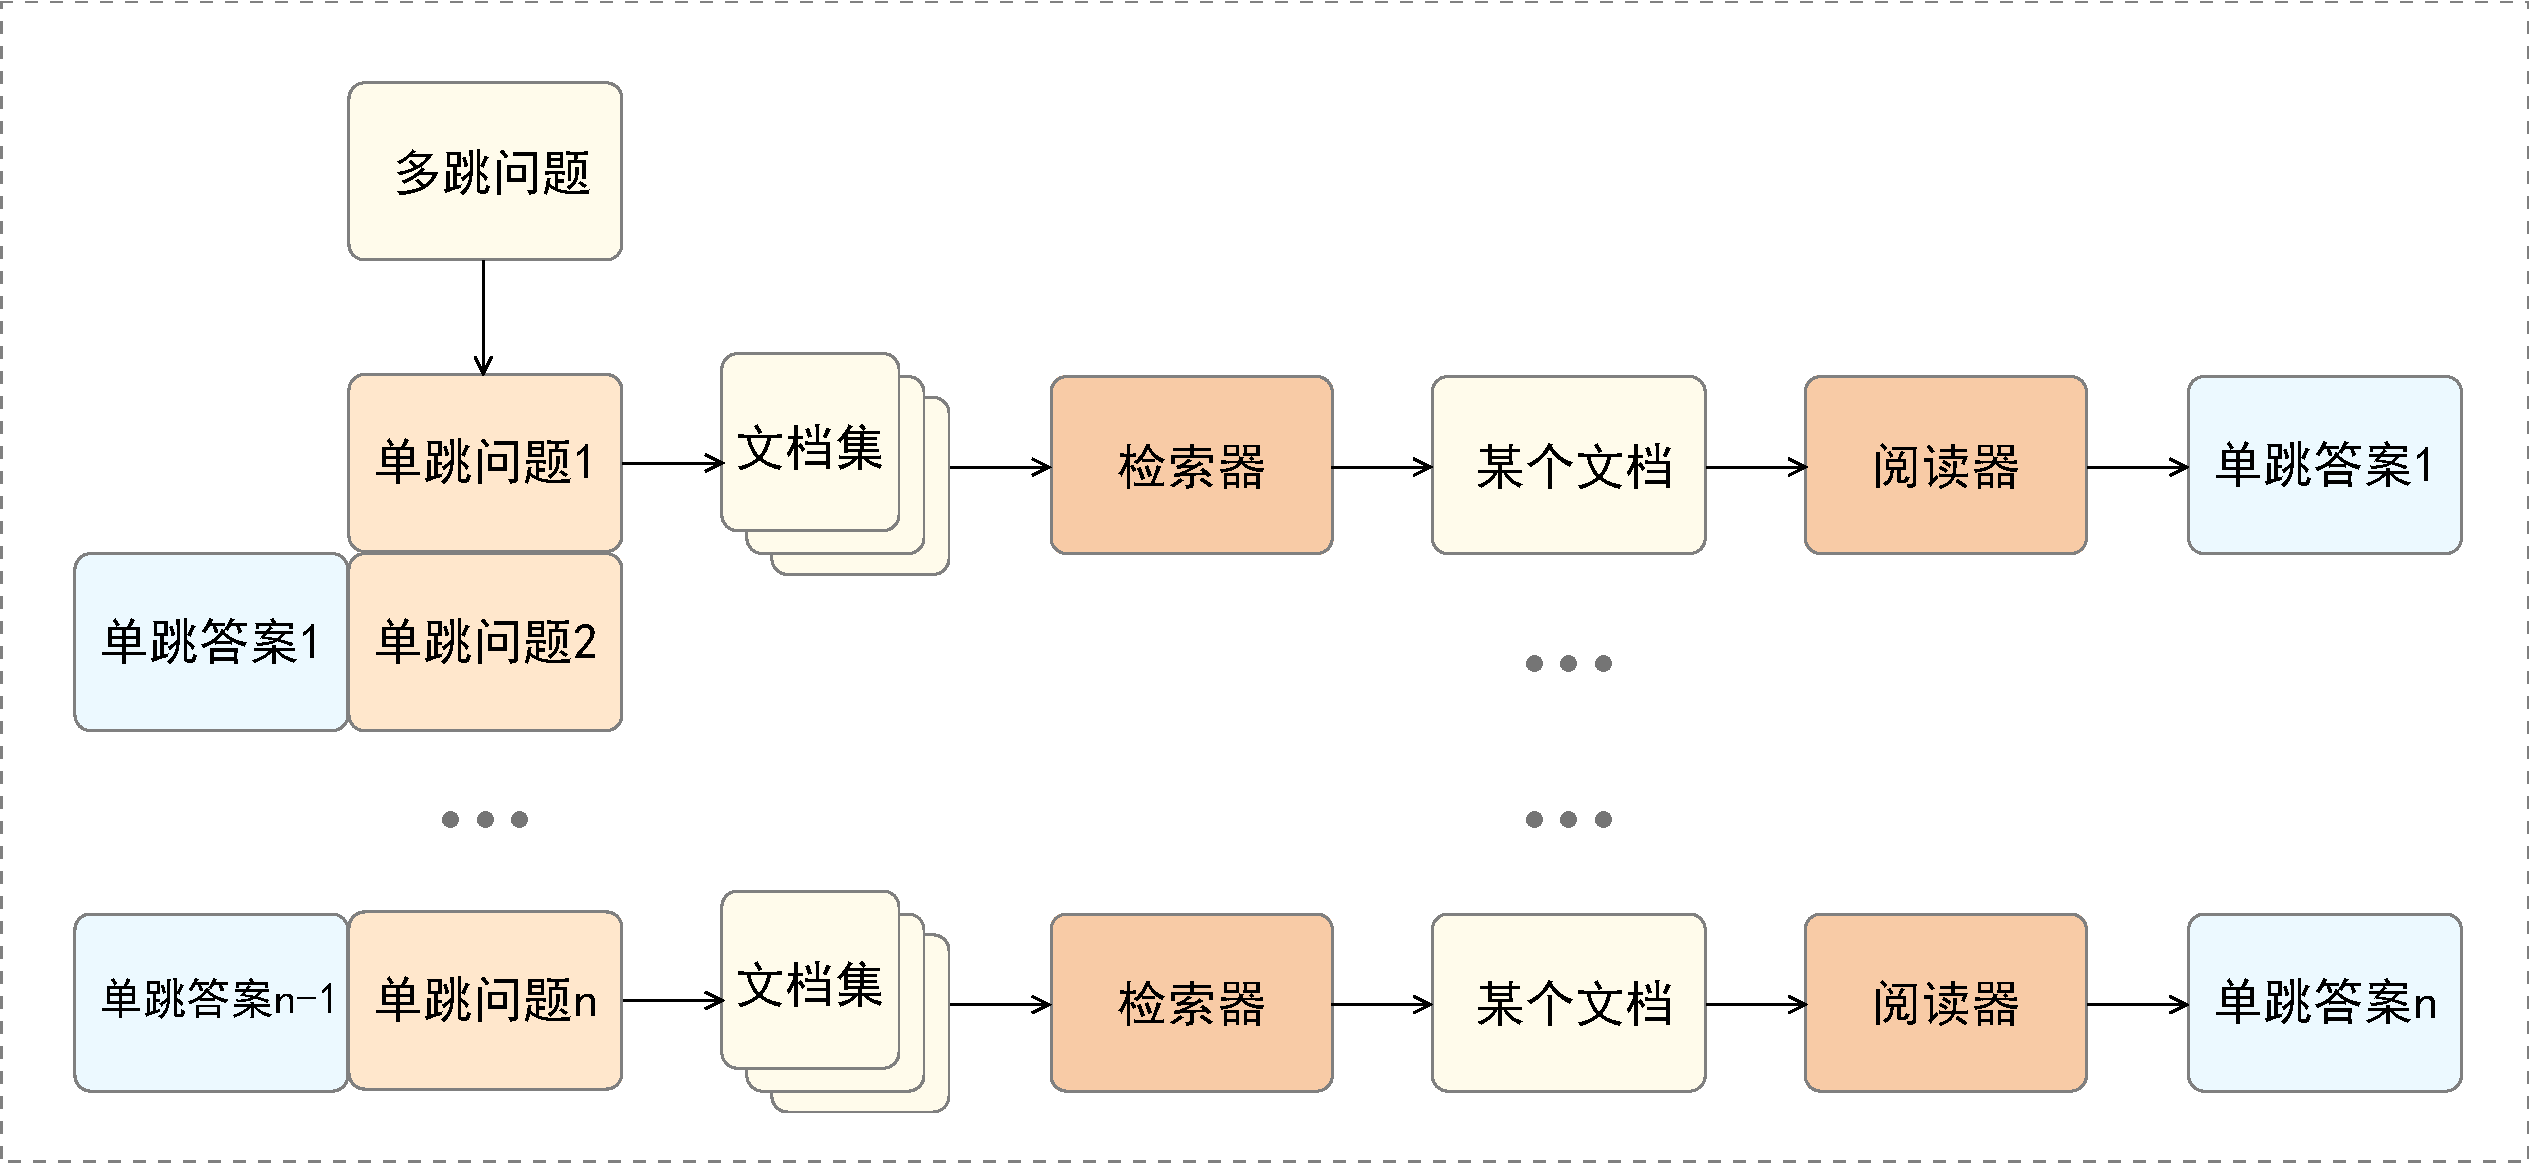
\includegraphics [width=1.0\textwidth] {figure/5-1.pdf}
    \caption{SeqDecomposer的整体架构} 
    \label{fig:5-1}
\end{figure}



\subsection{基于序列到序列生成的问题分解模块}
% 为什么要使用问题分解技术?
问题分解技术可以将一个复杂的多跳问题拆分成多个简单的单跳问题。
这种方法的好处是简化了问题的回答过程,使得回答过程更加可控和可解释。

% 怎么做的
本文首先提出SeqDecomposer架构,该架构对于多跳问题$Q$,采用序列到序列的生成模型,将$Q$分解为多个单跳问题$q_1,q_2,...,q_n$。
这个过程可以表示为:
\begin{equation}
    q_1,q_2,...,q_n = GEN(Q)
\end{equation}
序列到序列的生成模型通常有BART,T5等。
其中BART(Bidirectional and Auto-Regressive Transformer)是Facebook AI Research在2019年提出的一种序列到序列的生成模型模型。
其特点是可以同时进行自编码和自回归,可以在不同的任务中共享参数。
而T5(Text-to-Text Transfer Transformer)是Google在2020年提出的一种序列到序列的生成模型。
其特点是可以将所有的自然语言处理任务都转化为文本到文本的转换任务,从而可以用同一种模型来解决不同的任务。
本文同时使用了BART和T5,作为整个模型结构的一部分。
值得注意的是,从模型生成第二个及以后的子问题$q_i(i>=2)$开始,由于$q_i$可能需要$q_{i-1}$的答案$a_{i-1}$,因此在生成子问题$q_i$时,需要先将先前的答案$a_{i-1}$以词槽的形式填充到子问题$q_{i-1}$中。
直到整个系统得到最后一个子问题$q_{n}$的答案$a_{n}$后,整个系统的迭代将停止。

\subsection{基于预训练语言模型的阅读理解模型}
% 浅谈检索和阅读理解
在多跳阅读理解中,参考文本一般以多文档的形式给出。
这种形式决定了文档的总长度会特别长,因此,类似于第三章中对长文本的处理方式,本章也需要针对每个单跳问题,对文档进行检索和阅读的操作。

% 如何检索单跳问题的相关文档
针对单跳问题$q_i$,由于$q_i$只能从特定文档中获取答案,因此首先需要检索模型,从所有备选文档中找到相关文档。
例如,在MuSiQue数据集中,对于大部分问题,总共分配20个文档,记为$D={D_1, D_2, ..., D_20}$,这20个文档中只有一个文档与$q_i$是相关的。
本节的做法是将子问题$q_i$与所有文档依次进行拼接,组合成$x_{ij}=[CLS]q_i[SEP]D_j[SEP]$的形式。
之后,通过一个预训练语言模型,来得到$x_{ij}$的整体表示,记为$H_{ij}$。
之后,一层全连接网络和Softmax层可以得到$H_{ij}$的分类概率值$\hat y_c$。
$\hat y_{ij}$可以理解为子问题$q_i$与文档$D_j$的相关性。
本文通过计算$\hat y_{ij}$与子问题$q_i$所对应的唯一正确文档标签$y_{ij}$之间的损失,来监督检索模型的学习。
其中,检索出与子问题$q_i$相关的文档的交叉熵损失函数可以表示为:
\begin{equation}
    \mathcal  L^{Retr}_{i}  = -y_{ij}\log\hat y_{ij}+(1-y_{ij})log(1-\hat y_{ij})
\end{equation}

% 如何抽取单跳问题的答案
得到子问题$q_i$的相关文档$D_j$后,阅读模块需要再次将两者的表示拼接在一起,得到$x_i=[CLS]q_i[SEP]D_j[SEP]$。
然后,阅读模块中的编码器将$x_i$转化成隐向量;
该隐向量经过一个指针网络,可以标识出文档中每个token作为答案起始位置和结束位置的概率值,分别用$\hat y_s$和$\hat y_e$来表示。
训练过程中,用真实答案的起始和结束位置$y_s$和$y_e$来进行训练,其损失函数可以表示为:
\begin{equation}
    \mathcal L^{Ans}_{i} = \frac{1}{2} CrossEntropy(\hat y_s,y_s) + \frac{1}{2} CrossEntropy(\hat y_e,y_e)
\end{equation}

% 如何将子答案融入到下一个单跳问题中
在推理阶段,如果上述模型得到的子答案$a_i$不是最后一跳问题的答案,应该将它填充到下一个单跳问题$q_{i+1}$中,填充$q_{i+1}$中的槽位。
如此,下一跳问题$q_{i+1}$成为了一个完整的用自然语言描述的问题,可以循环执行检索与阅读的步骤,从而得到最后一跳的答案$a_n$。

\subsection{基于分步执行的问题分解技术}
% 前面的问题分解模式有什么缺点?为什么要改进?
上一小节描述的SeqDecomposer架构,通过序列到序列的生成模型,将复杂的多跳问题一次性分解为了一些列单跳问题。
尽管子问题用占位符临时填充单跳问题,让每个问题看上去具备连贯性。
然而本文认为,这种做法在生成子问题的过程中,并没有充分使用可利用的答案信息。

% 新的问题分解的做法
为此,本节稍稍改动了SeqDecomposer的工作流程,提出一种不同的架构StepDecomposer。
StepDecomposer相比于SeqDecomposer只在问题分解的部分作出了改动。
对于复杂的多跳问题$Q$,StepDecomposer每次只让生成模型生成一个单跳问题$q_i$。
具体如图图~\ref{tab:5-2}~所示,对于问题$Q$和已经生成好的前$k-1$跳单跳问题$q_1, q_2, ..., q_{k-1}$,这些单跳问题已经通过前述的检索和阅读理解模型得到了对应的子答案$a_1, a_2, ..., a_{k-1}$。
此时,把这些已知信息,包括原始问题$Q$,单跳问题$q_1, q_2, ..., q_{k-1}$以及单跳答案$a_1, a_2, ..., a_{k-1}$输入给生成式模型,目标是生成下一跳问题$q_k$,即:
\begin{equation}
    q_k = GEN(Q,q_1,a_1,q_2,a_2,...,q_{k-1},a_{k-1})
\end{equation}
在生成最后一跳问题$q_n$后,通过检索模型和阅读理解模型得到最终答案,即为完成了整个流程。
值得注意的是,由于在现实应用中,多跳问题的跳数是无法事先得知的。
因此,本文为QuALITY训练集中的最后一跳问题打好了结束标记。
如此一来,当生成式模型生成出的问题带上了结束标记时,代表此时已经来到了最后一跳问题。

% % 整体任务结构
\begin{figure}[htbp]
    \centering
    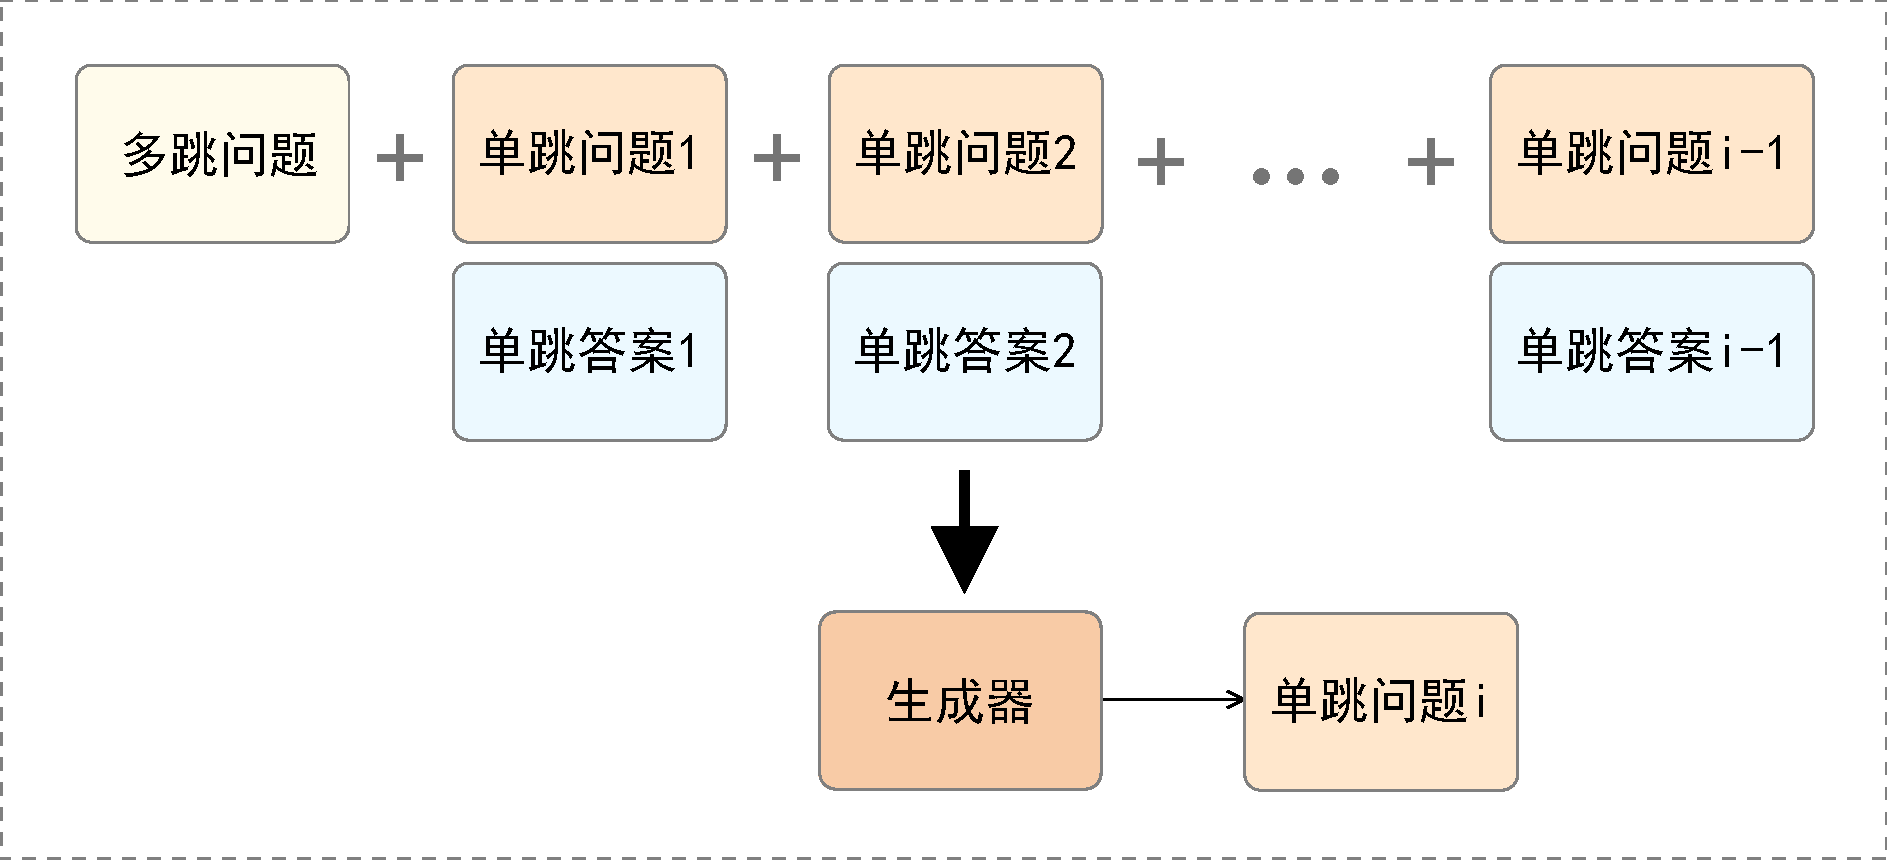
\includegraphics [width=0.8\textwidth] {figure/5-2.pdf}
    \caption{StepDecomposer的问题分解过程} 
    \label{fig:5-2}
\end{figure}



\section{实验及结果分析}

\subsection{实验设置}
% 数据集简介
本章在多跳多文档阅读理解数据集MuSiQue上进行了大量实验。
MuSiQue的文章主要来源于英文维基百科,具体来说,它是一些经典的阅读理解数据集做了重构,例如SQuAD等。
MuSiQue中对于每个问题所给出的问题,要远远大于其他多跳数据集。
数据集中\%99以上的问题,都给出了20个可能相关的文档。
此外,有少部分问题是给出了16-19个文档。
MuSiQue中包含了2-4跳总共约25k个问题,其中2跳问题占据了绝大多数。
而训练集则是包含了20k个问题。
不同于以往的多跳阅读理解数据集,MuSiQue往往是需要给出正确的多跳支持证据才能找到最终答案。
由于实验过程涉及到问题分解,所以本文还统计了MuSiQue中问题的长度分布。
在训练集中,多跳问题的token数量中位数为18;
经过训练好的生成模型将它分解为多个单跳问题后,其拼接后的句子的token数量的中位数为28。

% Baseline介绍

% 超参数设定

\subsection{实验结果和分析}
% 问题分解部分的实验

% 问题分解部分的实验分析

% 主实验
阅读器F1(5C)

% 消融实验
检索器ACC(5D)


\section{本章小结}

本章提出了一种基于问题分解技术,用以处理多跳阅读理解任务的方法,并改善模型搜寻支持证据的能力。
该方法分为SeqDecomposer和StepDecomposer两种类型,它们都主张将复杂的多跳问题分解为多个简单的单跳问题。
然后利用这些单跳问题,依次完成检索和阅读理解任务。
实验结果和分析表明,该方法在捕获证据文档的能力上有可观的提升。
然而,本章仍未全方位的生成模型进行探索。
因此,未来的研究会考虑应用大模型中思维链的方式,来对问题分解做更细致的研究。


